\documentclass[a4paper]{article}

\usepackage[pdftex]{graphicx}
\usepackage[margin=3cm]{geometry}
\usepackage{verbatim,moreverb,amssymb,amsmath}


\newcounter{question}
\newcommand{\question}[1]{\refstepcounter{question}\section*{Question~\thequestion~~~\small\emph{(#1)}}}
\renewcommand*\thequestion{\arabic{question}}


\begin{document}

\pagestyle{empty}
\thispagestyle{empty}



\noindent
\begin{minipage}{\columnwidth}
  \centering
  \Large
  DA4002 (HT13) Halmstad University\\
  Introduction to Algorithms, Data Structures, and Problem Solving\\[3\baselineskip]
  \Huge
  Written Exam\\
  \Large
  Friday, November 1, 2013\\[2\baselineskip]
  Examiner: Roland Philippsen
\end{minipage}

\vfill

\noindent
\begin{center}
\fbox{
  \begin{minipage}{0.8\columnwidth}
    \textbf{Student Name:}\\[3\baselineskip]
  \end{minipage}
}
\end{center}

\vfill



\section*{Rules}

Aside from the obvious rules of conduct exams (e.g.\ no chatting):

\begin{itemize}
\item
  \textbf{No computing devices} (laptops, phones, calculators, \emph{etc}).
\item
  \textbf{No books or printouts} except for non-electronic dictionaries.
\item
  \textbf{Allowed hand-written notes}: two sheets of A4 paper (front and back).
\end{itemize}



\section*{General Guidelines}

\begin{itemize}
\item
  \textbf{Read carefully} and pace yourself.
  You can solve the problems in any order you want, but later problems may be easier to solve after you have answered the preceding questions.
\item
  \textbf{Write clearly} and draw clear diagrams.
  If you need to correct a mistake, then cleanly cross out the wrong answer and clearly indicate where the correction can be found.
\item
  \textbf{Indicate the question number} for each of your answers.
  If a question has sub-questions, indicate the sub-question number after the main question number, separated by a dot.
  For example, question 3 has 4 sub-questions, and their answers should be numbered 3.1, 3.2, 3.3, and 3.4.
\end{itemize}



\pagebreak
\pagestyle{plain}
\thispagestyle{plain}
\setcounter{page}{1}



\question{6 points}

Match the data structure names with the diagrams \textbf{(A)}, \textbf{(B)}, \textbf{(C)}, and the code segments \textbf{(X)}, \textbf{(Y)}, and \textbf{(Z)}.

\begin{center}
  \begin{tabular}{|l|*2{p{0.2\columnwidth}|}}
    \hline
    \emph{data structure} & \emph{diagram (A, b, or C)} & \emph{code (X, Y, or Z)} \\
    \hline
    & & \\
    \textbf{simply} linked list & & \\
    & & \\
    \hline
    & & \\
    \textbf{doubly} linked list & & \\
    & & \\
    \hline
    & & \\
    \textbf{binary} tree & & \\
    & & \\
    \hline
    & & \\
    \textbf{k-ary} tree & & \\
    & & \\
    \hline
    & & \\
    \textbf{undirected} graph & & \\
    & & \\
    \hline
    & & \\
    directed \textbf{acyclic} graph & & \\
    & & \\
    \hline
  \end{tabular}
\end{center}

%\begin{center}
%  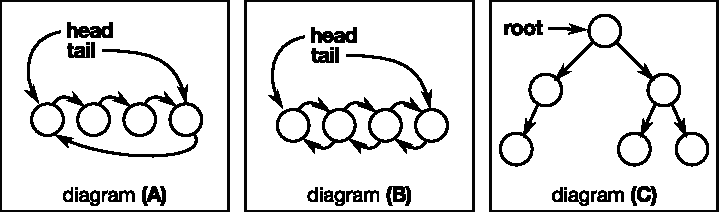
\includegraphics[width=0.6\columnwidth]{q1diag.pdf}
%\end{center}



\clearpage


\question{6 points}

Give them recursive code for the coin change problem, let them develop and fill out the DP variant.



\clearpage

\question{6 points}

Determine big-Oh expressions for a two $T$ expressions (iterative and recursive) and two code segments (iterative and recursive).



\clearpage

\question{6 points}

Do a bunch of runtime estimates given big-Oh expressions.

(add table with $x^2$ etc)



\clearpage

\question{6 points}

Give an adjacency matrix, let them draw the graph, describe Dijkstra, let them run it on the graph they drew.



\clearpage

\question{6 points}

Hmm\ldots unbalanced tree problem is always a good one, and I don't think I have trees yet.
Or something to do with tree traversal\ldots



\end{document}
